% Copyright 2004 by Till Tantau <tantau@users.sourceforge.net>.
%
% In principle, this file can be redistributed and/or modified under
% the terms of the GNU Public License, version 2.
%
% However, this file is supposed to be a template to be modified
% for your own needs. For this reason, if you use this file as a
% template and not specifically distribute it as part of a another
% package/program, I grant the extra permission to freely copy and
% modify this file as you see fit and even to delete this copyright
% notice. 

\documentclass{beamer}

% There are many different themes available for Beamer. A comprehensive
% list with examples is given here:
% http://deic.uab.es/~iblanes/beamer_gallery/index_by_theme.html
% You can uncomment the themes below if you would like to use a different
% one:
%\usetheme{AnnArbor}
%\usetheme{Antibes}
%\usetheme{Bergen}
%\usetheme{Berkeley}
%\usetheme{Berlin}
%\usetheme{Boadilla}
%\usetheme{boxes}
%\usetheme{CambridgeUS}
%\usetheme{Copenhagen}
%\usetheme{Darmstadt}
%\usetheme{default}
%\usetheme{Frankfurt}
%\usetheme{Goettingen}
%\usetheme{Hannover}
%\usetheme{Ilmenau}
%\usetheme{JuanLesPins}
%\usetheme{Luebeck}
\usetheme{Madrid}
%\usetheme{Malmoe}
%\usetheme{Marburg}
%\usetheme{Montpellier}
%\usetheme{PaloAlto}
%\usetheme{Pittsburgh}
%\usetheme{Rochester}
%\usetheme{Singapore}
%\usetheme{Szeged}
%\usetheme{Warsaw}
\usepackage{xcolor}
\setbeamercovered{transparent}
\usepackage{amsmath}
\usepackage{eucal}
\usepackage{graphics}
\usepackage[justification=centering]{caption}
\usepackage[utf8]{inputenc}
\usepackage[T1]{fontenc}
\usepackage[francais]{babel}

\defbeamertemplate*{footline}{mytheme}
{
    \leavevmode%
          \hbox{%
              \begin{beamercolorbox}[wd=.3\paperwidth,ht=2.25ex,dp=1ex,center]{section in head/foot}%
                  \usebeamerfont{author in head/foot}~{Mohammed~Khatiri}
              \end{beamercolorbox}%
              \begin{beamercolorbox}[wd=.4\paperwidth,ht=2.25ex,dp=1ex,center]{section in head/foot}%
                  \usebeamerfont{author in head/foot}~\insertshorttitle{}
              \end{beamercolorbox}%
              \begin{beamercolorbox}[wd=.3\paperwidth,ht=2.25ex,dp=1ex,right]{section in head/foot}%
                  \usebeamerfont{date in head/foot}
                  \insertframenumber{} / \inserttotalframenumber\hspace*{2ex} 
              \end{beamercolorbox}}%
                  \vskip0pt%
              }
\usebeamertemplate{mytheme}



\title{Les architectures Microservices}

% A subtitle is optional and this may be deleted
\subtitle{id\'ee g\'en\'erale et avantages}

\author{Mohammed~Khatiri\inst{2}\inst{1}}
% - Give the names in the same order as the appear in the paper.
% - Use the \inst{?} command only if the authors have different
%   affiliation.

\institute[Univ. Grenoble Alpes, CNRS, Inria, LIG] % (optional, but mostly needed)
{
    \inst{1}%
  University Mohammed First\\
  Faculty of Sciences, LaRI, Morocco\\
  \textcolor{red}{Professeur El Mostafa DAOUDI}
  \and
  \inst{2}%
  Univ. Grenoble Alpes\\
  CNRS, Inria, LIG, France \\
  \textcolor{red}{Professeur Denis trystram}}
% - Use the \inst command only if there are several affiliations.
% - Keep it simple, no one is interested in your street address.

\date{Séminaires - LaRI \\ 28-05-2018 }
% - Either use conference name or its abbreviation.
% - Not really informative to the audience, more for people (including
%   yourself) who are reading the slides online

%\subject{Theoretical Computer Science}
% This is only inserted into the PDF information catalog. Can be left
% out. 

% If you have a file called "university-logo-filename.xxx", where xxx
% is a graphic format that can be processed by latex or pdflatex,
% resp., then you can add a logo as follows:

% \pgfdeclareimage[height=0.5cm]{university-logo}{university-logo-filename}
% \logo{\pgfuseimage{university-logo}}

% Delete this, if you do not want the table of contents to pop up at
% the beginning of each subsection:
\AtBeginSubsection[]
{
    \begin{frame}<beamer>{Outline}
        \tableofcontents[currentsection,currentsubsection]
    \end{frame}
}

% Let's get started
\begin{document}

\begin{frame}
    \titlepage
\end{frame}

\begin{frame}{Outline}
    \tableofcontents
    % You might wish to add the option [pausesections]
\end{frame}

% Section and subsections will appear in the presentation overview
% and table of contents.

%\section{Objectives}

%\begin{frame}{Objectives de Cette Pr\'esentation}
%    \begin{itemize}[<+->]
%        \item {
 %               Pr\'esentation des architectures - Monolithique - Microservices.              
 %           }\\ 
 %       \item 
 %               Architectures des Microservices : 
 %           \begin{itemize}
 %%               \item Principe
 %               \item Isolation des Microservices
 %               \item Machines virtuelles VS conteneurs
  %              \item Communication entre les Microservices
  %          \end{itemize}
  %                    
 %       \item Avantage des Microservices
 %           \begin{itemize}
 %               \item D\'eploiement
 %               \item Mises \'a jour
 %               \item Bugs d\'ecentralis\'ee 
 %               \item Scalabilit\`e
 %           \end{itemize}
 %%
 %%       \item Inconv\`enients (Limites) des architectures Microservices.
 %           \begin{itemize}
 %               \item Taille des services 
 %               \item Système de supervision
 %           \end{itemize}
%
%        \item {
%            Conclusion
 %           }
 %
 %   \end{itemize}
%end{frame}
 %
 %
\section{Les architectures Monolithique}
\subsection{Les architectures Monolithique VS les architectures des Microservices}
\begin{frame}{Les architectures Monolithique}
    \begin{columns}
        \column{0.4\textwidth}
        \begin{figure}
            \begin{center}
            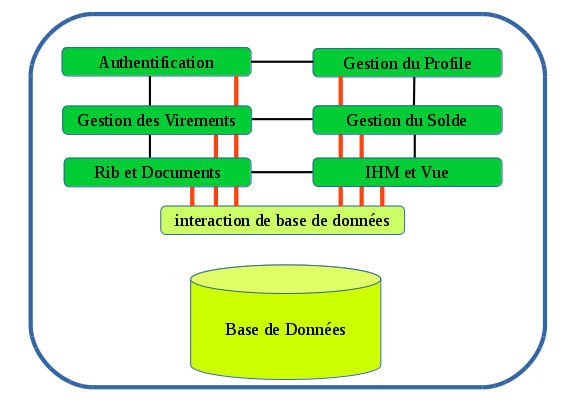
\includegraphics[width=1\textwidth]{monopolitique.png}
                \caption{Exemple d'application de banque \textcolor{red}{Architectures Monolithique}}
            \end{center}
        \end{figure}
        \column{.6\textwidth}
        Principe
        \begin{itemize}
            \item Un gros code contenant toutes les fonctionnalités et les
                différentes couches logicielles.
            \item les services communiquent à travers des appels de fonctions 
            \item Une seule grosse compilation et un seul livrable (un gros fichier WAR)
            \item Une seule pile logicielle (Linux, JVM, Tomcat Présentation et bibliothèques tierces)
        \end{itemize} 
    \end{columns}

                %\includegraphics[width=0.5\textwidth]{imonopolitique.pn}
\end{frame}

\section{Les architectures des Microservices}
% Placing a * after \section means it will not show in the
% outline or table of contents.
\subsection*{Principe}
\begin{frame}{Les architectures des Microservices}
    \begin{itemize}
     \item Premières discussions autour du terme microservice en 2011 lors d’un workshop sur les architectures logicielles
    \item une évolution des architectures orientées services
    \begin{columns}
        \column{0.4\textwidth}
        \begin{figure}
            \begin{center}
            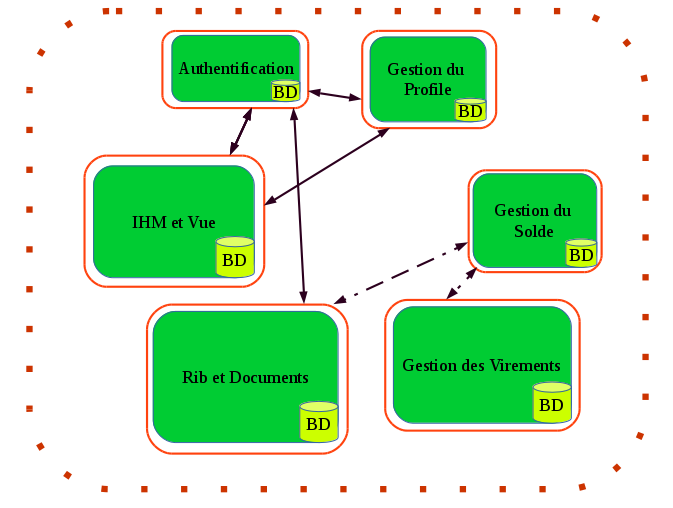
\includegraphics[width=1\textwidth]{Microservices.png}
                \caption{Exemple d'application de banque \textcolor{red}{Architectures Microservices}}
            \end{center}
        \end{figure}
        \column{.6\textwidth}
        Principe :
        \begin{itemize}
            \item Un ensemble de microservices autonomes.
            \item Chaque Microservices réalise une seule fonctionnalité de
                l'application globale.
            \item Un microservice possède un contexte d’exécution séparé
                des autres. \alert{isolation}
            \item Les Microservices communiquent à travers le réseau. 
                \begin{itemize}
                    \item Communication synchrone : services web (\alert{SOAP} ou \alert{REST})
                    \item Communication asynchrone : les bus d’événements 
                \end{itemize}
        \end{itemize} 
    \end{columns}
    \end{itemize}
\end{frame}

\subsection{Isolation des Microservices}

\begin{frame}{Isolation des Microservices}
\begin{itemize}
         \item Un Microservices doit être séparé de l'application globale. 
         \item Cette technique consiste à isoler l’utilisation des ressources de type processeur, mémoire et disque par application sur une même machine.
         \item Un microservice peut contenir toutes les couches logicielles (IHM, middleware et base de données)
         \item Comment on peut fait \alert{l'isolation} ??????
             \begin{itemize}
                 \item Virtualisation.
                 \item \alert{Machines virtuelles}.
                 \item \alert{Conteneurs}.
             \end{itemize}
\end{itemize}
\end{frame}

\subsection*{Machines virtuelles VS conteneurs}
\begin{frame}{Machines virtuelles VS conteneurs}
    \begin{center}  Le mode de fonctionnement \end{center}
    \begin{columns}
        \column{0.5\textwidth}
        \textbf{ Machine virtuelle :} 
        \begin{itemize}
            \item Représente un ordinateur complet 
            \item Un système d’exploitation(SE) complet avec les pilotes et des des systèmes de fichiers binaires
            \item L’application
        \end{itemize}
            \begin{center}
           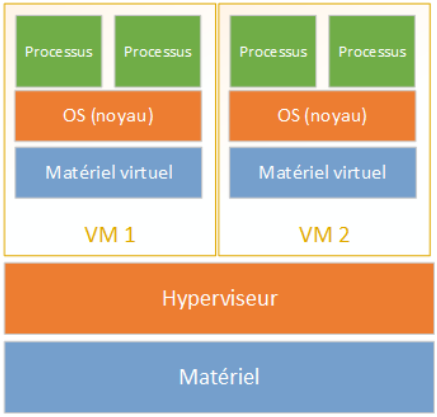
\includegraphics[width=35mm,height=30mm]{VM.png}
            \end{center}
        \column{0.5\textwidth}
        \textbf{Conteneurs}
        \begin{itemize}
            \item Une image de base composée d’un SE.
            \item L'application
        \end{itemize}
        % \begin{figure}
            \begin{center}
                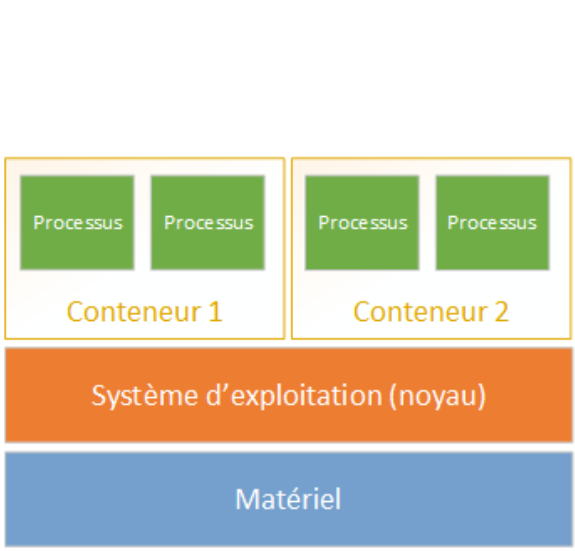
\includegraphics[width=35mm,height=40mm]{Conteneures.png}
           %     \caption{Exemple d'application de banque \textcolor{red}{Architectures Microservices}}
            \end{center}
       % \end{figure}

    \end{columns}

\end{frame}

\begin{frame}{Machines virtuelles VS conteneurs}
    \begin{center}  Le différence entre les machines virtuelles et les conteneurs \end{center}
    \begin{columns}
        \column{0.5\textwidth}
        \textbf{ Machine virtuelle :} 
        \begin{itemize}
            \item S’exécute dans un environnement isolé de virtualisation 
                matérielle grâce à un hyperviseur 
            \item Tous les éléments exécutés dans une VM sont
                masqués du SE hôt 
            \item Apparaît comme un ordinateur physique.
            \item Très lourde lors de démarrage.
        \end{itemize}
        \column{0.5\textwidth}
        \textbf{Conteneurs}
        \begin{itemize}
            \item Ne nécessite pas d’hyperviseur pour assurer son 
            \item utilise les fonctionnalités d’isolation des processus et du système de fichier du noyau linux.
            \item Le conteneur paraît comme une instance unique du système d’exploitation.
            \item Le temps de démarrage et la surcharge d'espace sont réduits. 
        \end{itemize}
    \end{columns}

\end{frame}

\begin{frame}{Machines virtuelles VS conteneurs}
    \begin{center}  Les différence sur les performances
    \end{center}
         \begin{figure}
            \begin{center}
                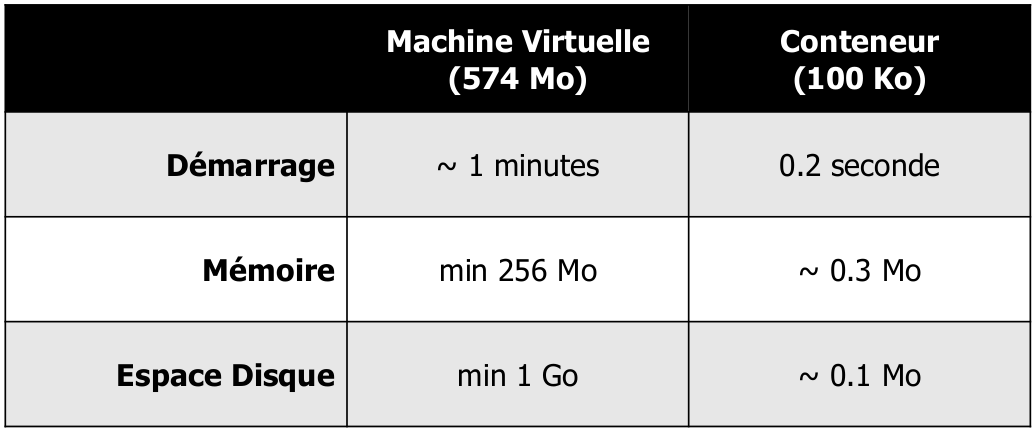
\includegraphics[width=1\textwidth]{performances.png}
            \end{center}
        \end{figure}
\end{frame}

\subsection{Les outils}
\begin{frame}{Les outils}
    \begin{itemize}
        \item \textbf{les Microservices : } langage selon le besoin.
        \item \textbf{Isolation :} Docker
        \item \textbf{Image système : } \href{https://hub.docker.com/}{\beamergotobutton{://hub.docker.com/}}
        \item \textbf{Communication } 
            \begin{itemize}
                \item \textbf{Synchrone : } HTMLi-JS, POST/GET, SOAP.
                \item \textbf{Asynchrone : } RabbitMQ
            \end{itemize}
        \item \textbf{Automatiser le déploiement sur clusters :} Kubernetes 
    \end{itemize}
\end{frame}
\section{Exemple de HELLO WORLD}
\begin{frame}{Exemple HELLO WORLD - Résumer }   
         \begin{figure}
            \begin{center}
                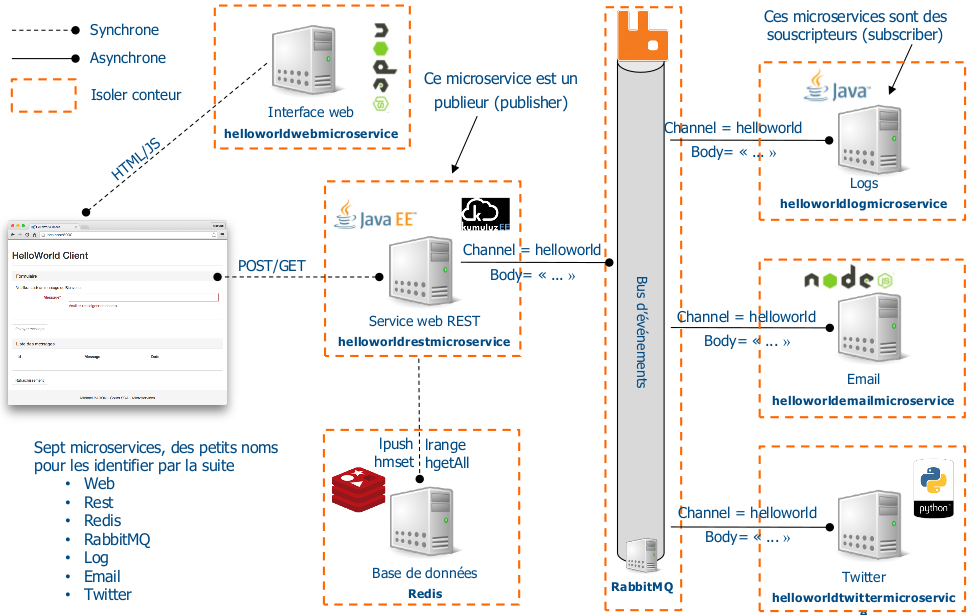
\includegraphics[width=0.9\textwidth]{hello.png}
            \end{center}
        \end{figure}
\end{frame}



\section{Avantage des Microservices }
\subsection{Mises à jour}
\begin{frame}{Mises à jour ou Maintenance }
    \begin{columns}
        \column{0.5\textwidth}
        \textbf{Applications Monolithique :} 
                \begin{itemize}
                    \item Mise à jours ou Maintenance d'un service nécessite la mise a jour de toute l'application.
                    \item Redémarrer tout application.
                \end{itemize}
        \begin{figure}
            \begin{center}
            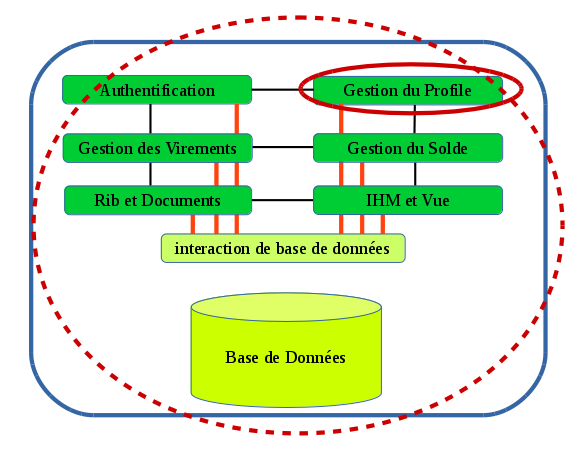
\includegraphics[width=0.88\textwidth]{MAJmono.png}
            \end{center}
        \end{figure}
        \column{0.5\textwidth}
        \pause
        \textbf{Applications avec Microservices :}
         \begin{itemize}
                    \item Mise à jours d'un Microservice ne nécessite pas la mise a jour de toute l'application.
                    \item lancer juste la nouvelle 'instance du Microservice concerné.
                     \item L'application ne s'arrête pas
                \end{itemize}
        \begin{figure}
            \begin{center}
            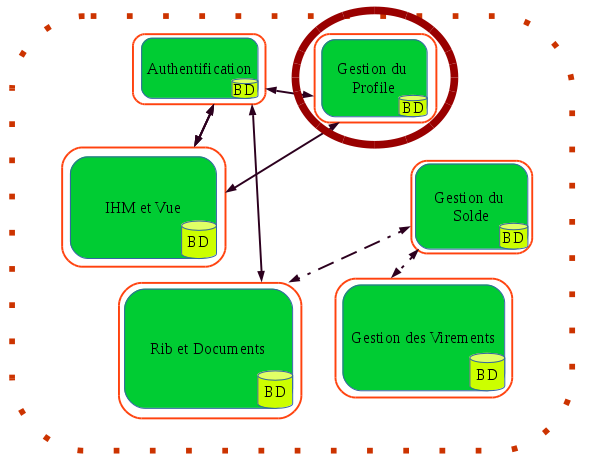
\includegraphics[width=0.6\textwidth]{MAJMicroservices.png}
            \end{center}
        \end{figure}
        

    \end{columns}
    
\end{frame}
\subsection{Bugs d\'ecentralis\'ee}
\begin{frame}{Bugs}
    \begin{columns}
        \column{0.5\textwidth}
        \textbf{Applications Monolithique :} 
                \begin{itemize}
                    \item l'interruption d'un service implique l'interruption de toute l'application.
                \end{itemize}
        \begin{figure}
            \begin{center}
            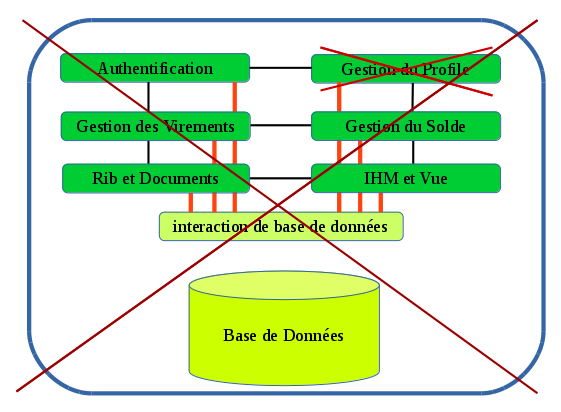
\includegraphics[width=0.8\textwidth]{BUGmono.png}
            \end{center}
        \end{figure}
        \column{0.5\textwidth}
        \pause
        \textbf{Applications avec Microservices :}
         \begin{itemize}
                    \item l'interruption d'un service n'affecte pas toutes les applications.
                \end{itemize}
        \begin{figure}
            \begin{center}
            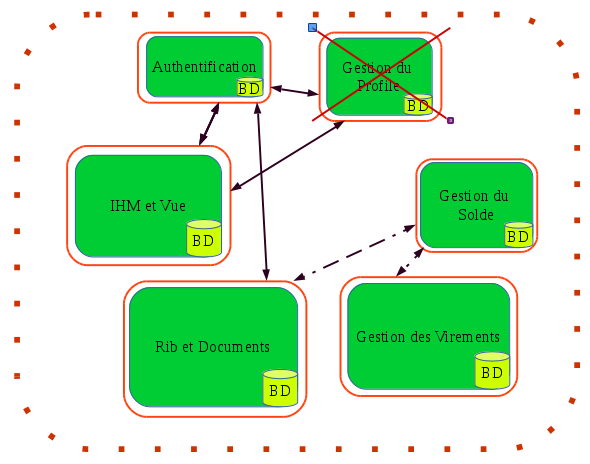
\includegraphics[width=0.8\textwidth]{BUGMicroservices.png}
            \end{center}
        \end{figure}
        

    \end{columns}
    
\end{frame}
\subsection{Consommation de ressources et Scalabilit\`e}
\begin{frame}{Consommation de ressources et Scalabilit\`e}
        \textbf{Applications Monolithique :}
        \begin{itemize}
            \item Supposons que l'application est déployée sur \alert{6 nœuds} de calcul
            \item Même catégorie de clients pour l'application (quelle que soit la demande) 
            \item Si le nombre de clients augmente : 
                \begin{itemize}
                    \item dupliquer l'application sur les machines et diviser le travail entre les deux instances
                    \item + \alert{6 nœuds} de calcul
                \end{itemize}
        \end{itemize}
        \pause
        \textbf{Applications avec Microservices : }
        \begin{itemize}
            \item Supposons que l'application est déployée sur \alert{6 nœuds} de calcul \alert{(Chaque nœuds prend un Microservice)}
            \item Les clients sont catégorisés en fonction des Microservices demandés
            \item Si le nombre d'utilisateurs augmente : 
                \begin{itemize}
                    \item Besoin de savoir quel microservict est chargé?
                    \item dupliquer Juste le microservice charger
                    \item + \alert{1 ou 2 nœuds} de calcul
                \end{itemize}
        \end{itemize}
\
\end{frame}

\section{Inconv\`enients (Limites) des architectures Microservices.}
\subsection{Inconv\`enients (Limites) des architectures Microservices}
    \begin{frame}{Les limites des architectures Microservices}
        \textbf{Taille des services}\\
        Le plus grand principe des microservices concerne la taille de ces services.
        \begin{itemize} 
            \item Pas de règles précises ou norme ou de spécification.
            \item Il est donc important de trouver un juste milieu entre des services imposants et des services trop petits
        \end{itemize} 
        \textbf{la supervision}
        \begin{itemize}
            \item La multiplicité des services entraîne une complexification de la supervision du système.
            \item le nombre de services croît régulièrement au fur et à mesure de la vie du système. 
            \item Il devient vite impossible pour un humain de suivre tous les services manuellement
            \item Des règles d’alertes automatiques doivent être mises en
                place afin de savoir lorsqu’un service
                commence à ne plus fonctionner correctement
            \item \alert{Le rôle du kubernetes sur les clouds (mais la configuration est manuel)}
        \end{itemize} 
    \end{frame}

\section{Qui utilisent les microservices ?}
\subsection{Qui utilisent les microservices ?}
\begin{frame}{Qui utilisent les microservices ?}
    \begin{itemize}
        \item Uber : https://eng.uber.com/soa/
        \item Netflix : http://techblog.netflix.com/
        \item Amazon : http://fr.slideshare.net/apigee/i-love-apis-2015-microservices-at-amazon
        \item Le prochain Eclipse Che IDE
    \end{itemize} 
\end{frame}

\section{Conclusion}
\subsection{Développer des architectures microservice ?}
    \begin{frame}{Développer des architectures microservice ?}
        \begin{itemize} 
            \item Savoir \textbf{Isoler} un microservice.
            \item Savoir \textbf{Coder} le contenu du microservice.
            \item Savoir faire \textbf{Communiquer} des microservices.
            \item Savoir \textbf{Composer} les microservices.
            \item Savoir \textbf{Répartir} les charges.
        \end{itemize}

    \end{frame}
\subsection{Conclusion}
    \begin{frame}{Conclusion}
        \begin{itemize} 
            \item la différence entre les architectures  
                Monolithique est Microservices.
            \item Principe d'isolation (Machine virtuel ou conteneurs)
            \item Les outils nécessaire
            \item Les avantages et les limites des architectures Microservices.
        \end{itemize}

    \end{frame}
\begin{frame}
    \begin{center}
    Merci de votre présence\\
        \textbf{Question ?}
    \end{center}
\end{frame}

\end{document}



